\documentclass[11pt]{article}

\usepackage{fullpage}
\usepackage{graphicx}
\graphicspath{ {./} }
\setlength{\parindent}{0pt}

\begin{document}

\title{ARM Checkpoint Report}
\author{J. Bae, A. Reynaldi, R. Rusly, P. Mazurina}

\maketitle

\section{Emulator Implementation}
\begin{figure}[h]
  \centering
  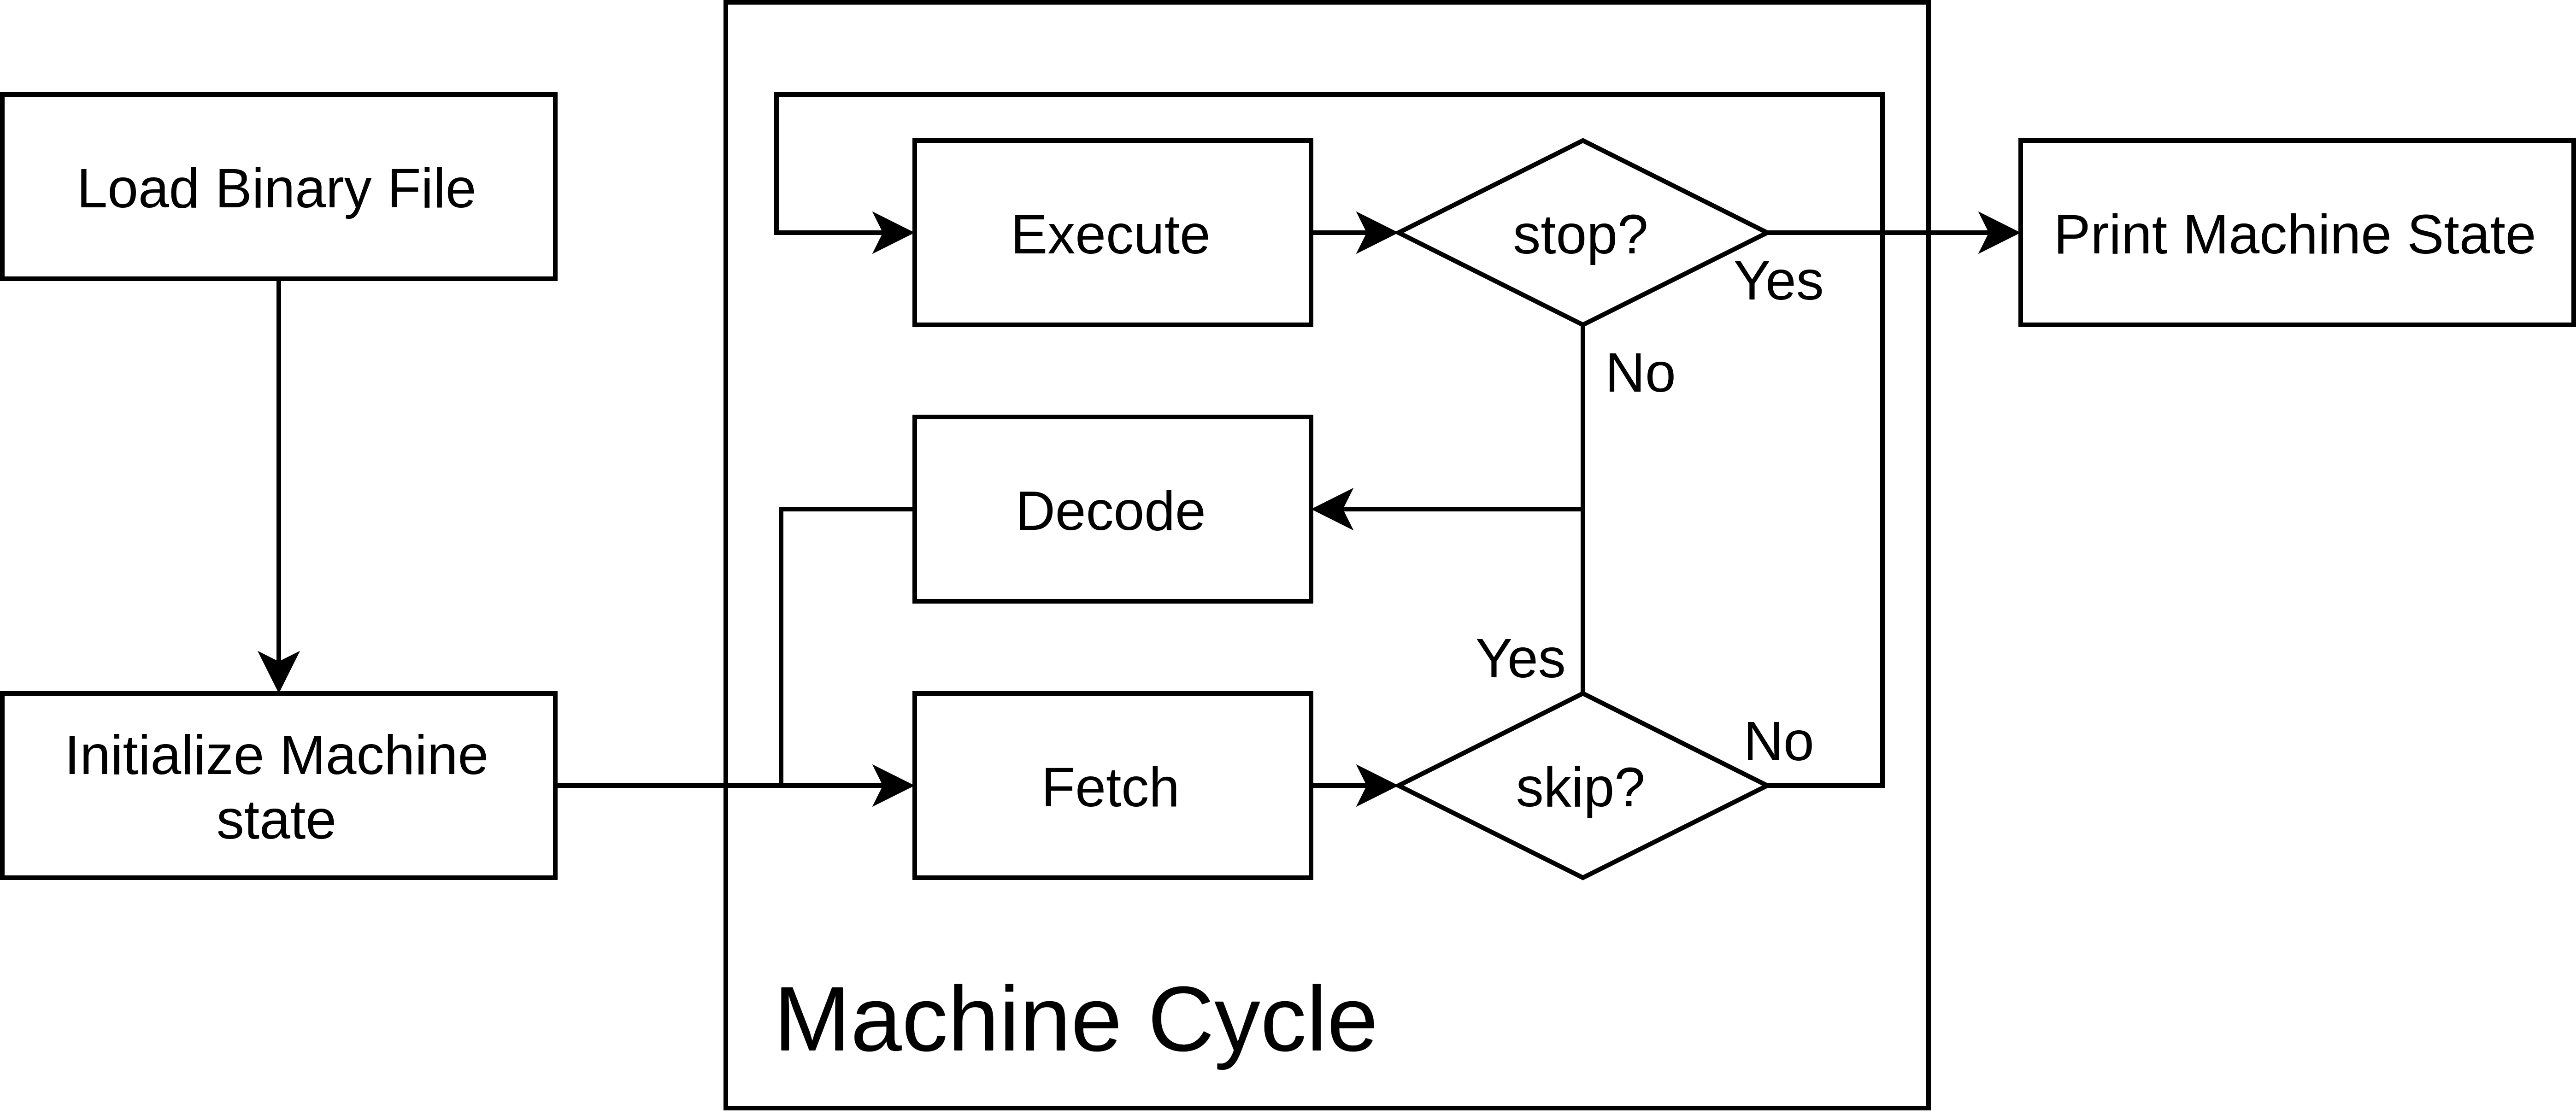
\includegraphics[width=0.7\linewidth]{emulator_structure.png}
  \caption{High-level representation of emulator structure.}
\end{figure}
The cycle is entered from Fetch, because in the first cycle nothing is decoded
or executed. We initalised skip to true so that the second cycle skips
execution as intended. Afterwards, skip is set whenever a jump instruction is
executed, effectively refreshing the pipeline. The machine state and the
decoded instruction are passed to execute. These are represented using structs:
\begin{itemize}
    \item \textbf{Machine State Struct}. The machine state struct contains a
    pointer to emulated memory (which is a byte array on the heap) and to the
    registers (which is an int array on the heap). The emulated memory is
    loaded with the contents of the binary file.
    \item \textbf{Instruction Structs}. Each of the 4 instruction types are
    represented by a struct that contains a list of words representing each
    operand of an instruction (e.g. for branch, this would mean 2 words: cond
    and offset). In Execute, we transform the instruction word into a struct of
    the correct type, before passing it to the execute function for that
    corresponding instruction type. We believe these structs will be reusable
    in the assembler as a buffer to hold operand values, before re-encoding
    them back into 32-bit word form.
\end{itemize}

In addition to the above, we wrote small utility functions to help with error
handling, bit fiddling and file loading. These can be reused for the assembler
as well. For more details on the program logic, see the Appendix.

\section{Challenging Sections}

We anticipated that implementing the machine cycle would be the most difficult
part of the emulator. Because this section is highly dependent on the
execution of the instructions, it is not easy to test. Hence, this task is
designated as a 2-person job, so that discussion and closer scrutiny could
prevent mistakes. The result of this is the Machine Cycle component represented
in the flowchart.

\bigskip
For Part II, we expect the symbol table ADT to be the most difficult section
to implement. Luckily, the symbol table is decoupled from the rest of the
program, and we can write unit tests for it. It will also be an important part
of our extension, as we are planning to build a compiler for an esoteric
programming language.
\section{Group Organisation}

We started the group project by splitting the emulator into individual tasks.
We then ordered our tasks appropriately, taking into account the availability
of each group member. The following diagram shows the task order and assignment:
\begin{itemize}
    \item Binary File Loader - Alex
    \item Machine State + printing - Rania
    \item Machine Cycle - Alex \& Rania
    \item Execute Data Processing - Polina
    \item Execute Multiply - Junhyuk
    \item Execute Single Data Transfer - Junhyuk
    \item Execute Branch - Alex
\end{itemize}

To ensure the quality of code and maintain discussion between group members,
we followed a code review process:
\begin{enumerate}
    \item When starting a task, start a new branch.
    \item Make commits to the task branch, making sure to check for any new
    changes to main that affect your code.
    \item When finished, create a merge request to master and assign to
    another group member.
    \item The other member suggests changes (either via text message or
    via comments on gitlab).
    \item If there are changes to be made, go to step 2. Otherwise, complete
    the merge and repeat with next task.
\end{enumerate}
In addition to the above, we hold weekly meeting calls on Microsoft Teams.
During the calls we split our tasks and discussed code implementations,
keeping track of them in a shared file. While these were effective, they were
difficult to arrange due to each member's different timezone. Some members'
preoccupations have also prevented them from completing their work on time.
Moving forward, we will need to communicate much more frequently and
efficiently to ensure we can finish by the deadline.
\newpage
\section{Appendix}
\subsection{Program Logic Details}
The following explains what each part of the program performs:
\begin{enumerate}
    \item Load binary file into memory
    \begin{enumerate}
        \item Open file specified by file name.
        \item Load file content into a BYTE array.
        \item If the verbose setting is on, prints the memory content
        in a format similar to xxd.
    \end{enumerate}
    \item Initialize Machine State
    \begin{enumerate}
        \item Initialize an int array containing register values.
        \item Create a struct containing pointers to memory and register array,
        where memory is the BYTE array previously mentioned.
    \end{enumerate}
    \item Machine Cycle
    \begin{enumerate}
        \item Fetch: load an instruction from M[PC] to the "fetched" buffer
        and increment PC by 4.
        \item Decode: convert fetched instruction from BYTE[4] to a WORD,
        and store it in the "decoded" buffer. Note that we do not perform an
        actual decoding here because it is simpler and more efficient to keep
        the instruction in encoded form.
        \item Execute: Create an instruction struct out of the "decoded"
        instruction. Note that this is where the actual decode takes place.
        Pass this struct to the appropriate execute function, along with the
        machine state. Return a SKIP, STOP, or CONTINUE signal depending on
        what instruction was executed and whether it was successful.
    \end{enumerate}
    \item Execution of Instructions
    \begin{enumerate}
        \item Data Processing: WIP
        \item Multiplication: WIP
        \item Single Data Transfer: WIP
        \item Branch: Check if cond is satisfied. If so, shift the offset to
        the left by 2 bits and sign extend it to 32 bits, and add the result
        the PC. If cond is not satisfied or the new PC exceeds the memory space,
        return a fail signal. Otherwise return a success signal.
    \end{enumerate}
\end{enumerate}
\end{document}
